\section{РЕАЛИЗАЦИЯ}
\addcontentsline{toc}{section}{Реализация}

\subsection{Обработка вызова метода API}

Алгоритм начинает свою работу с получения списка параметров, которые нужно передать в метод для его выполнения. Это возможно сделать с использованием reflectMethod, который предоставляет PHP. При отсутствии целевого метода кидается ошибка. Реализация данного шага приведена в листинге ~\ref{lst:api1}:


\begin{lstlisting}[caption={Код получения списка параметров, необходимых для передачи в метод API}, label=lst:api1]
// loop through the parameters 
// of the function being called
foreach($reflectMethod->getParameters() 
    as $i => $param) {
  $defaultAvailable = 
    $param->isDefaultValueAvailable();
  $parameterName = $param->getName();
  if($defaultAvailable) {
    $default = $param->getDefaultValue();
    if(($paramType = gettype($default)) == 'array') {
      // match this parameter of the function 
      // being called to the array
      // that was passed, if any (see above)
      $parameterName = '__array__';
    }
  }
}
\end{lstlisting}

Следующим шагом алгоритм сравнивает список необходимых параметров для метода и параметров, которые были переданы, а также происходит приведение типов. Если не был передан хотя бы один обязательный параметр - кидается ошибка с соответсрвующим описанием. Иначе происходит подстановка необязательных параметров, для которых установлено значение по умолчанию и не было передано значение.
Данный шаг приведен в листинге ~\ref{lst:api2}:

\begin{lstlisting}[caption={Код сравнения типов параметров}, label=lst:api2]
// loop through the parameters 
// of the function being called
foreach($reflectMethod->getParameters() 
    as $i => $param) {
  $defaultAvailable = 
    $param->isDefaultValueAvailable();
  $parameterName = $param->getName();
  if($defaultAvailable) {
    $default = $param->getDefaultValue();
    if(($paramType = 
        gettype($default)) == 'array') {
      $parameterName = '__array__';
    }
  }

  if(array_key_exists($parameterName, 
      $passedParams)) {
    // this parameter of the function being 
    // called was passed in the named parameters
    $val = $passedParams[$parameterName];
    $methodParams[] = $val;
    $params[] = "$parameterName = $val";;
  } elseif($defaultAvailable) {
    // parameter was not passed, 
    // assign a default value
    $methodParams[] = $default;
    $methodParamNames[] = $parameterName;
  } else {
    // parameter was not passed and no 
    // default value exists, trigger an error
    throw new \Exception
      ("Missing parameter $parameterName");
  }
}
\end{lstlisting}

Если два предыдущих шага прошли без ошибок, значит что соответвующий метод найден, и все необходимые параметры были переданы корректно. Происходит вызов метода с подготовленными параметрами и возврат результата. Пример использования функции вызова метода, определенной в PHP, приведен в листинге ~\ref{lst:api3}:

\begin{lstlisting}[caption={Вызов метода с подготовленными параметрами}, label=lst:api3]
$params = implode(', ', $params);
$this->logger->log("invoked $n ($params)");
return call_user_func_array
  (array(&$this, $n), $methodParams);
\end{lstlisting}

\subsection{Реализация моделей для ORM}

Рассмотрим на физическом уровне модели, являющиеся хранилищами для основных бизнес-сущностей программного комплекса, таких как: Session, Webgate, Performance.

\subsection{Модель Session}

Модель Session является описанием одного сеанса мероприятия. Рассмотрим данные её модели, описаные на языке аннотаций Doctrine ORM:

\begin{lstlisting}
Webgate\MainBundle\Entity\Session:
  type: entity
  table: null
  indexes:
    - columns: [ date ]
    - columns: [ hidden ]
  fields:
    id:
      type: integer
      id: true
      generator:
        strategy: AUTO
    performance_id:
      type: string
      length: 255
    date:
      type: datetime
    available:
      type: boolean
    available_places_count:
      type: integer
      nullable: true
    min_price:
      type: integer
    max_price:
      type: integer
    hidden:
      type: boolean
    is_duplicate:
      type: boolean
    is_presentation:
      type: boolean
    last_update:
      type: datetime
  manyToOne:
    webgate:
      targetEntity: Webgate
      inversedBy: sessions
      joinColumn:
        onDelete: "CASCADE"
    webgate_performance:
      targetEntity: WebgatePerformance
      inversedBy: sessions
      joinColumn:
        onDelete: "CASCADE"
    hall:
      targetEntity: Hall
      inversedBy: sessions
  oneToMany:
    locked_places:
      targetEntity: LockedPlace
      mappedBy: session
  lifecycleCallbacks:
    preUpdate: [ preUpdate ]
\end{lstlisting}

Краткое описание полей модели Session:

performance --- мероприятие, к которому отностся данный сеанс;

date --- дата и время сеанса;

available --- доступна ли продажа билетов на данный сеанс;

available places count --- количество еще свободных мест;

min price, max price --- цены на билеты.

last update --- время последнего обновления модели данных;

\subsection{Модель Webgate}

Модель Webgate является описанием вебгейта, который обычно расположен удалённо. Рассмотрим описание данной модели:

\begin{lstlisting}
Webgate\MainBundle\Entity\Webgate:
  type: entity
  table: null
  indexes:
    - columns: [ limited ]
  fields:
    id:
      type: integer
      id: true
      generator:
        strategy: AUTO
    url:
      type: string
      length: 255
    name:
      type: string
      length: 255
    site:
      type: string
      length: 255
      nullable: true
    available:
      type: boolean
    limited:
      type: boolean
    checker_limited:
      type: boolean
    check_errors_count:
      type: integer
    unavailable_message:
      type: string
      length: 255
      nullable: true
  manyToOne:
    webgate_type:
      targetEntity: WebgateType
      inversedBy: webgates
      joinColumn:
        onDelete: "SET NULL"
  oneToMany:
    webgate_performances:
      targetEntity: WebgatePerformance
      mappedBy: webgate
    institutions:
      targetEntity: Institution
      mappedBy: webgate
    sessions:
      targetEntity: Session
      mappedBy: webgate
    orders:
      targetEntity: OrderInfo
      mappedBy: webgate
    users:
      targetEntity: WebgateUser
      mappedBy: webgate
  lifecycleCallbacks: {  }
\end{lstlisting}

Краткое описание полей модели Webgate:

url --- url, по которому доступен данный вебгейт;

available --- состояние вебгейта, работает ли он в данный момент;

limited --- запретить ли осуществление продаж для данного вебгейта;


\subsection{Схема базы данных}

В программном комплексе используется база данных MySQL версии 5.5. Фреймворк Symfony имеет встроенную ORM Doctrine, которая может автоматически генерировать таблицы в базе данных, используея описанные модели. На рисунке ~\ref{fig:db-schema} приведена схема базы данных.

\begin{figure}[H]
  	\centering
 	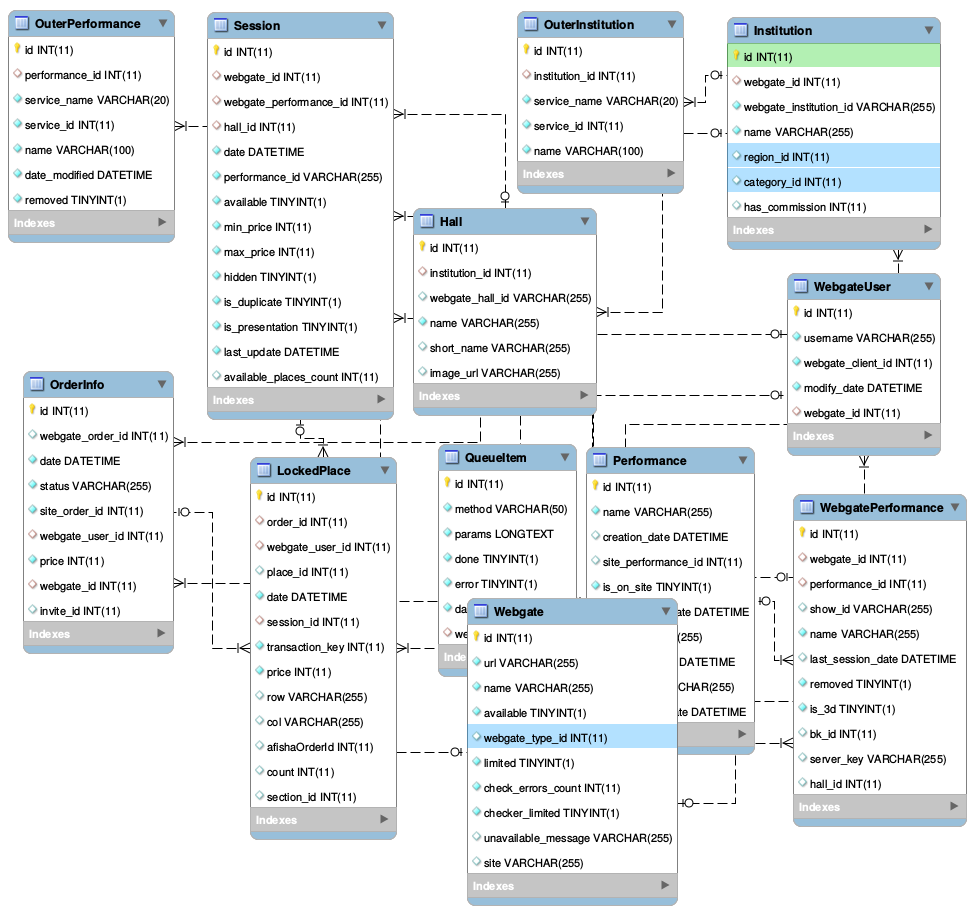
\includegraphics[width=0.8\textwidth]{images/db-schema.png}
  	\caption{Схема базы данных}
    \label{fig:db-schema}
\end{figure}

\subsection{Обработчик очереди запросов}

Обработчик очереди запросов выполняется отдельно для каждого вебгейта. С заранее заданной переодичностью обработчик выбирает порцию еще не обработанных запросов и передает их в метод обработки. Алгоритм выборки приведен в листинге ~\ref{lst:queue-algo}:

\begin{lstlisting}[caption={Алгоритм выборки запросов из очереди}, label=lst:queue-algo]
  $em = $this->getContainer()
    ->get('doctrine.orm.api_entity_manager');
  $q = $em->getRepository('WebgateMainBundle:QueueItem')
      ->createQueryBuilder('qi')
      ->where('qi.done = 0 AND qi.error = 0')
  ;
  if ($webgate_id = $input->getOption('webgate_id')) {
      $q = $q
          ->andWhere('qi.webgate = :webgate_id')
          ->setParameter('webgate_id', $webgate_id)
      ;
  }
  $qis = $q
      ->setMaxResults(20)
      ->getQuery()
      ->getResult()
  ;
  foreach($qis as $qi){
      $this->getContainer()
        ->get('queue_handler')
        ->handle($qi);
      $em->persist($qi);
      $em->flush();
  }
\end{lstlisting}


В листинге ~\ref{lst:handle-algo} приведен метод обработки одного запроса, переданного из обработчика очереди отложенных запросов. Делается попытка выполнить запрос. Любая ошибка, которая произошла во время исполняния вызваннного метода перехватывается, и запрос помечается как выполненный с ошибкой. В дальнейшем запросы, выполненный с ошибкой будут обработаны еще раз.

\begin{lstlisting}[caption={Алгоритм обработки выбранного запроса}, label=lst:handle-algo]
  public function handle(QueueItem $qi){
    $params = implode(', ', $qi->getParams());
    $this->logger->Log("Executing #{$qi->getId()} 
      {$qi->getMethod()} with params {$params}", 
      'queue.log', true);

    try{
      $method = $qi->getMethod();
      $this->$method($qi->getParams());
      $qi->setError(false);
      $qi->setDone(true);
    }catch(\Exception $e){
      $qi->setError(true);
      $qi->setDone(false);
      $this->logger->Log("Error while executing 
        #{$qi->getId()}: {$e->getMessage()}", 
        'queue.log', true);
    }
  }
\end{lstlisting}  


\newpage